%% Revisão da literatura

% ---
% Este capítulo, utilizado por diferentes exemplos do abnTeX2, ilustra o uso de
% comandos do abnTeX2 e de LaTeX.
% ---

\chapter{Revisão da Literatura}\label{rev_literatura}

Este capítulo tem como objetivo consolidar a linha de raciocínio fundamental para a elaboração dessa dissertação. Primeiramente
será apresentado um panorama geral sobre o agronegócio brasileiro, com foco na cultura do algodão, abordando pontos como os principais desafios da produção, 
suaa importância e seus destinos comerciais. Em seguida, detalha-se o processo de avaliação da qualidade do algodão, com ênfase nos padrões intenacionais,
regulamentações específicas no Brasil e os processos adotados na indústria. Na sequência, será contextualizado o tema dos sistemas de visão computacional,
com aplicações no setor da agricultura, especialemnte na classificação automatizada. Por fim, o capitulo discutirá o papel da inteligência artificial e 
os principais modelos empregados em sistemas de visão computacional.

\section{Agronegócio Brasileiro e o Algodão}\label{rev_agro_algodao}

A agricultura brasileira já se consolidou como uma das maiores do mundo, fornecendo produtos essenciais para diversos setores da economia 
global, como a alimentação, a bioenergia, o setor têxtil ente outros. Essa consolidação é um reflexo de investimentos em inovações tecnológicas, que começaram 
com a terceira revolução agrícola (Revolução Verde) e se estendem até hoje com a disseminação da agricultura digital, integrando a 
agricultura de precisão e ferramentas como inteligência artificial para aumento da produtividade e sustentabilidade \cite{abbade2014agro, basso2024agriculture}.

O setor tem se destacado como um dos mais robustos, representando 23\% da economia nacional \cite{filho2024pib}, com exportações atingindo recordes históricos. 
Mesmo em cenários de queda nos preços das commodities e desafios climáticos, como a seca e fenômenos como o El Niño \cite{lin2019elnino} e desafios logísticos \cite{goncalves2024logistica}, 
o Brasil manteve o crescimento no valor total exportado. Em 2024, a expectativa é de que o país alcance US\$ 168,1 bilhões em exportações de produtos 
agrícolas, impulsionado por fatores como a desvalorização do real frente ao dólar, o que aumenta a competitividade dos produtos
 brasileiros no mercado internacional \cite{cardoso2024perspectivas}.

No contexto da produção agrícola brasileira, a tecnologia desempenhou um papel essencial na adaptação do país a diferentes 
tipos de culturas, permitindo o cultivo de variedades mais resistentes e otimizadas para o clima tropical \cite{basso2024agriculture}. 
Além disso, a introdução de biotecnologia e o avanço em estudos moleculares têm possibilitado o desenvolvimento de culturas com maior 
produtividade e resistência a pragas \cite{das2023biotech}, sendo o algodão (\textit{Gossypium hirsutum}) um exemplo significativo e cuja produção 
se beneficia de tais avanços, como resistência genética e técnicas de cultivo adaptadas ao clima e solo brasileiros \cite{ribeiro2017cottontrans, ribeiro2019cottontrans, ribeiro2023cottontrans}.

Em 2024 o Brasil se consolidou como o maior exportador mundial de algodão em volume. As condições climáticas favoráveis, aliadas ao aumento da 
demanda internacional, permitiram um crescimento expressivo das exportações brasileiras de algodão em 2024. 
A produção alcançou 3,2 milhões de toneladas, com a China como principal destino, e as exportações estão projetadas para somar US\$ 5,2 bilhões 
até o fim do ano, um aumento de 56\% em relação ao ano anterior. Isso reflete o papel estratégico do algodão na pauta exportadora do agronegócio 
brasileiro, que vai além da alimentação, abrangendo setores como o têxtil e de bioenergia \cite{cardoso2024perspectivas}.

\begin{itemize}
	\item Agro no Brasil (produção do agro, importância do algodão)
	\item Algodão (história, destinação)
	\item Algodão no Brasil e no cerrado (desafios)
	\item Números economicos (Comercialização, principais importadores, etc.)
\end{itemize}

\section{Qualidade do Algodão}\label{rev_qualidade_algodao}

A classificação e a avaliação da qualidade do algodão são processos fundamentais para a cadeia de produção e comércio dessa fibra, influenciando diretamente o valor de mercado e a adequação às diversas aplicações industriais. Nesta seção será examinado o histórico, os critérios de classificação e as normas internacionais, com destaque para o sistema estadunidense, além das especificidades regulatórias no Brasil.

\subsection{Contexto histórico e econômico}

A prática sistemática de classificação do algodão remonta do início do século XIX, tendo como origem na cidade de
Liverpool na Inglaterra. A implementação dessa prática foi necessária devido à modernização das máquinas de fiar,
impulsionada na primeira revolução industrial, onde se observou que 
a eficiência na produção de fios era maior dependendo da qualidade da fibra, gerando assim mais lucro para o fiador
\cite{morais2021interpretacao}. As transações comerciais da fibra do algodão passaram então a levar em conta sua
qualidade, porém dependendo do setor envolvido (produtor ou fiador) a percepção sobre a qualidade
da fibra mudava. Assim, foram desenvolvidos padrões para unificar e facilitar a comercialização da fibra. 
Nesse contexto, a criação de uma terminologia padronizada e de critérios objetivos de avaliação 
tornou-se essencial para a negociação e, especialmente, para garantir uma base de comparação justa que facilitasse 
as transações internacionais \cite{earle1914classification}.

Confome abordado por \citeonline{conant1915us}, a adoção do \textit{United States Cotton Futures Act} pela Bolsa de Algodão de Nova York, que reformou as práticas de contratos futuros de algodão após pressões significativas, incluindo uma  ameaça de imposto proibitivo. A principal mudança introduzida foi a substituição de um sistema arbitrário de fixação de diferenças de preço entre diferentes tipos de algodão por um sistema baseado nas diferenças comerciais reais do mercado à vista. Esse novo sistema visava alinhar melhor os contratos futuros com a realidade do mercado, evitando distorções que prejudicavam tanto a proteção de \textit{hedge} quanto a confiança no mercado. O ato também introduziu medidas de identificação por tipo para os fardos entregues em contrato e a supervisão direta do governo, trazendo mais transparência e equidade ao processo de negociação.

\citeonline{earle1914classification} também trazem que nos Estados Unidos, o sistema oficial de classificação foi desenvolvido no início do século XX, com a contribuição de produtores, especialistas e representantes do governo, resultando na formulação de nove padrões oficiais estabelecidos pelo Departamento de Agricultura (USDA). Na década de 1960 o USDA iniciou as pesquisas para deselvolver métodos instrumentais de classificação, que culminaram na adoção da classificação por HVI (\textit{High Volume Instrument}) praticamente em toda a produção americana de algodão \cite{knowlton2005usda}. Atualmente, apenas em casos especiais e identificação de corpos estranhos que o algodão é classificado de forma manual, porém pesquisas continuam sendo desenvolvidas para que a classificação instrumental contemple todos os aspectos avaliados \cite{cottoninc2020classification}.

\subsection{Classificação do algodão no Brasil}

No Brasil, o procedimento para a classificação da pluma do algodão é estabelecido pela Instrução Normativa n. 24 de 2016 do Ministério da Agricultura e leva em consideração Padrões Físicos Universais, como a cor da fibra, a presença de folhas e impurezas, contaminação de matérias estranhas e o modo de beneficionamento do produto \cite{mapa2016}.

Tem início com o processo de amostragem, que leva em consideração os seguintes pontos:

\begin{itemize}
    \item A amostra pode ser realizada manualmente ou mecanicamente;
    \item De cada fardo deve-se extrair duas amostras de lados opostos (no mínimo 150 gramas cada). Cada uma dessas amostras será dividida no sentido longitudinal e essa metada adicionada à medade da outra amostra, formando assim duas amostras de trabalho. Uma será enviada para classificação visual e outra para classificação instrumental;
    \item As amostras devem ser manuseadas e acondicionadas em pacotes de forma a não descaracterizá-las ao longo do processo;
    \item O tamanho das amostras deve ter no mínimo 25 a 30 centímetros de comprimento, 13 a 15 centímetros de largura e 8 a 13 centímetros de espessura;
\end{itemize}

\subsubsection{Classificação visual}

Após, uma das amostras retiradas seguem para o processo de classificação visual. Neste processo é utilizado como referência os Padrões Físicos Universais, que consistem em caixas com 6 amostras de algodão, tendo como base os padrões americanos para os algodões "\textit{Upland}" e "\textit{Pima}", conforme exemplo na Figura \ref{fig_padrao_fisico}.

\begin{figure}[H]
	\caption{\label{fig_padrao_fisico}Exemplo do Padrão Físico Universal (51.5: Cor Abaixo da Média, Branco / Grau de Folhas 5)}
	\begin{center}
		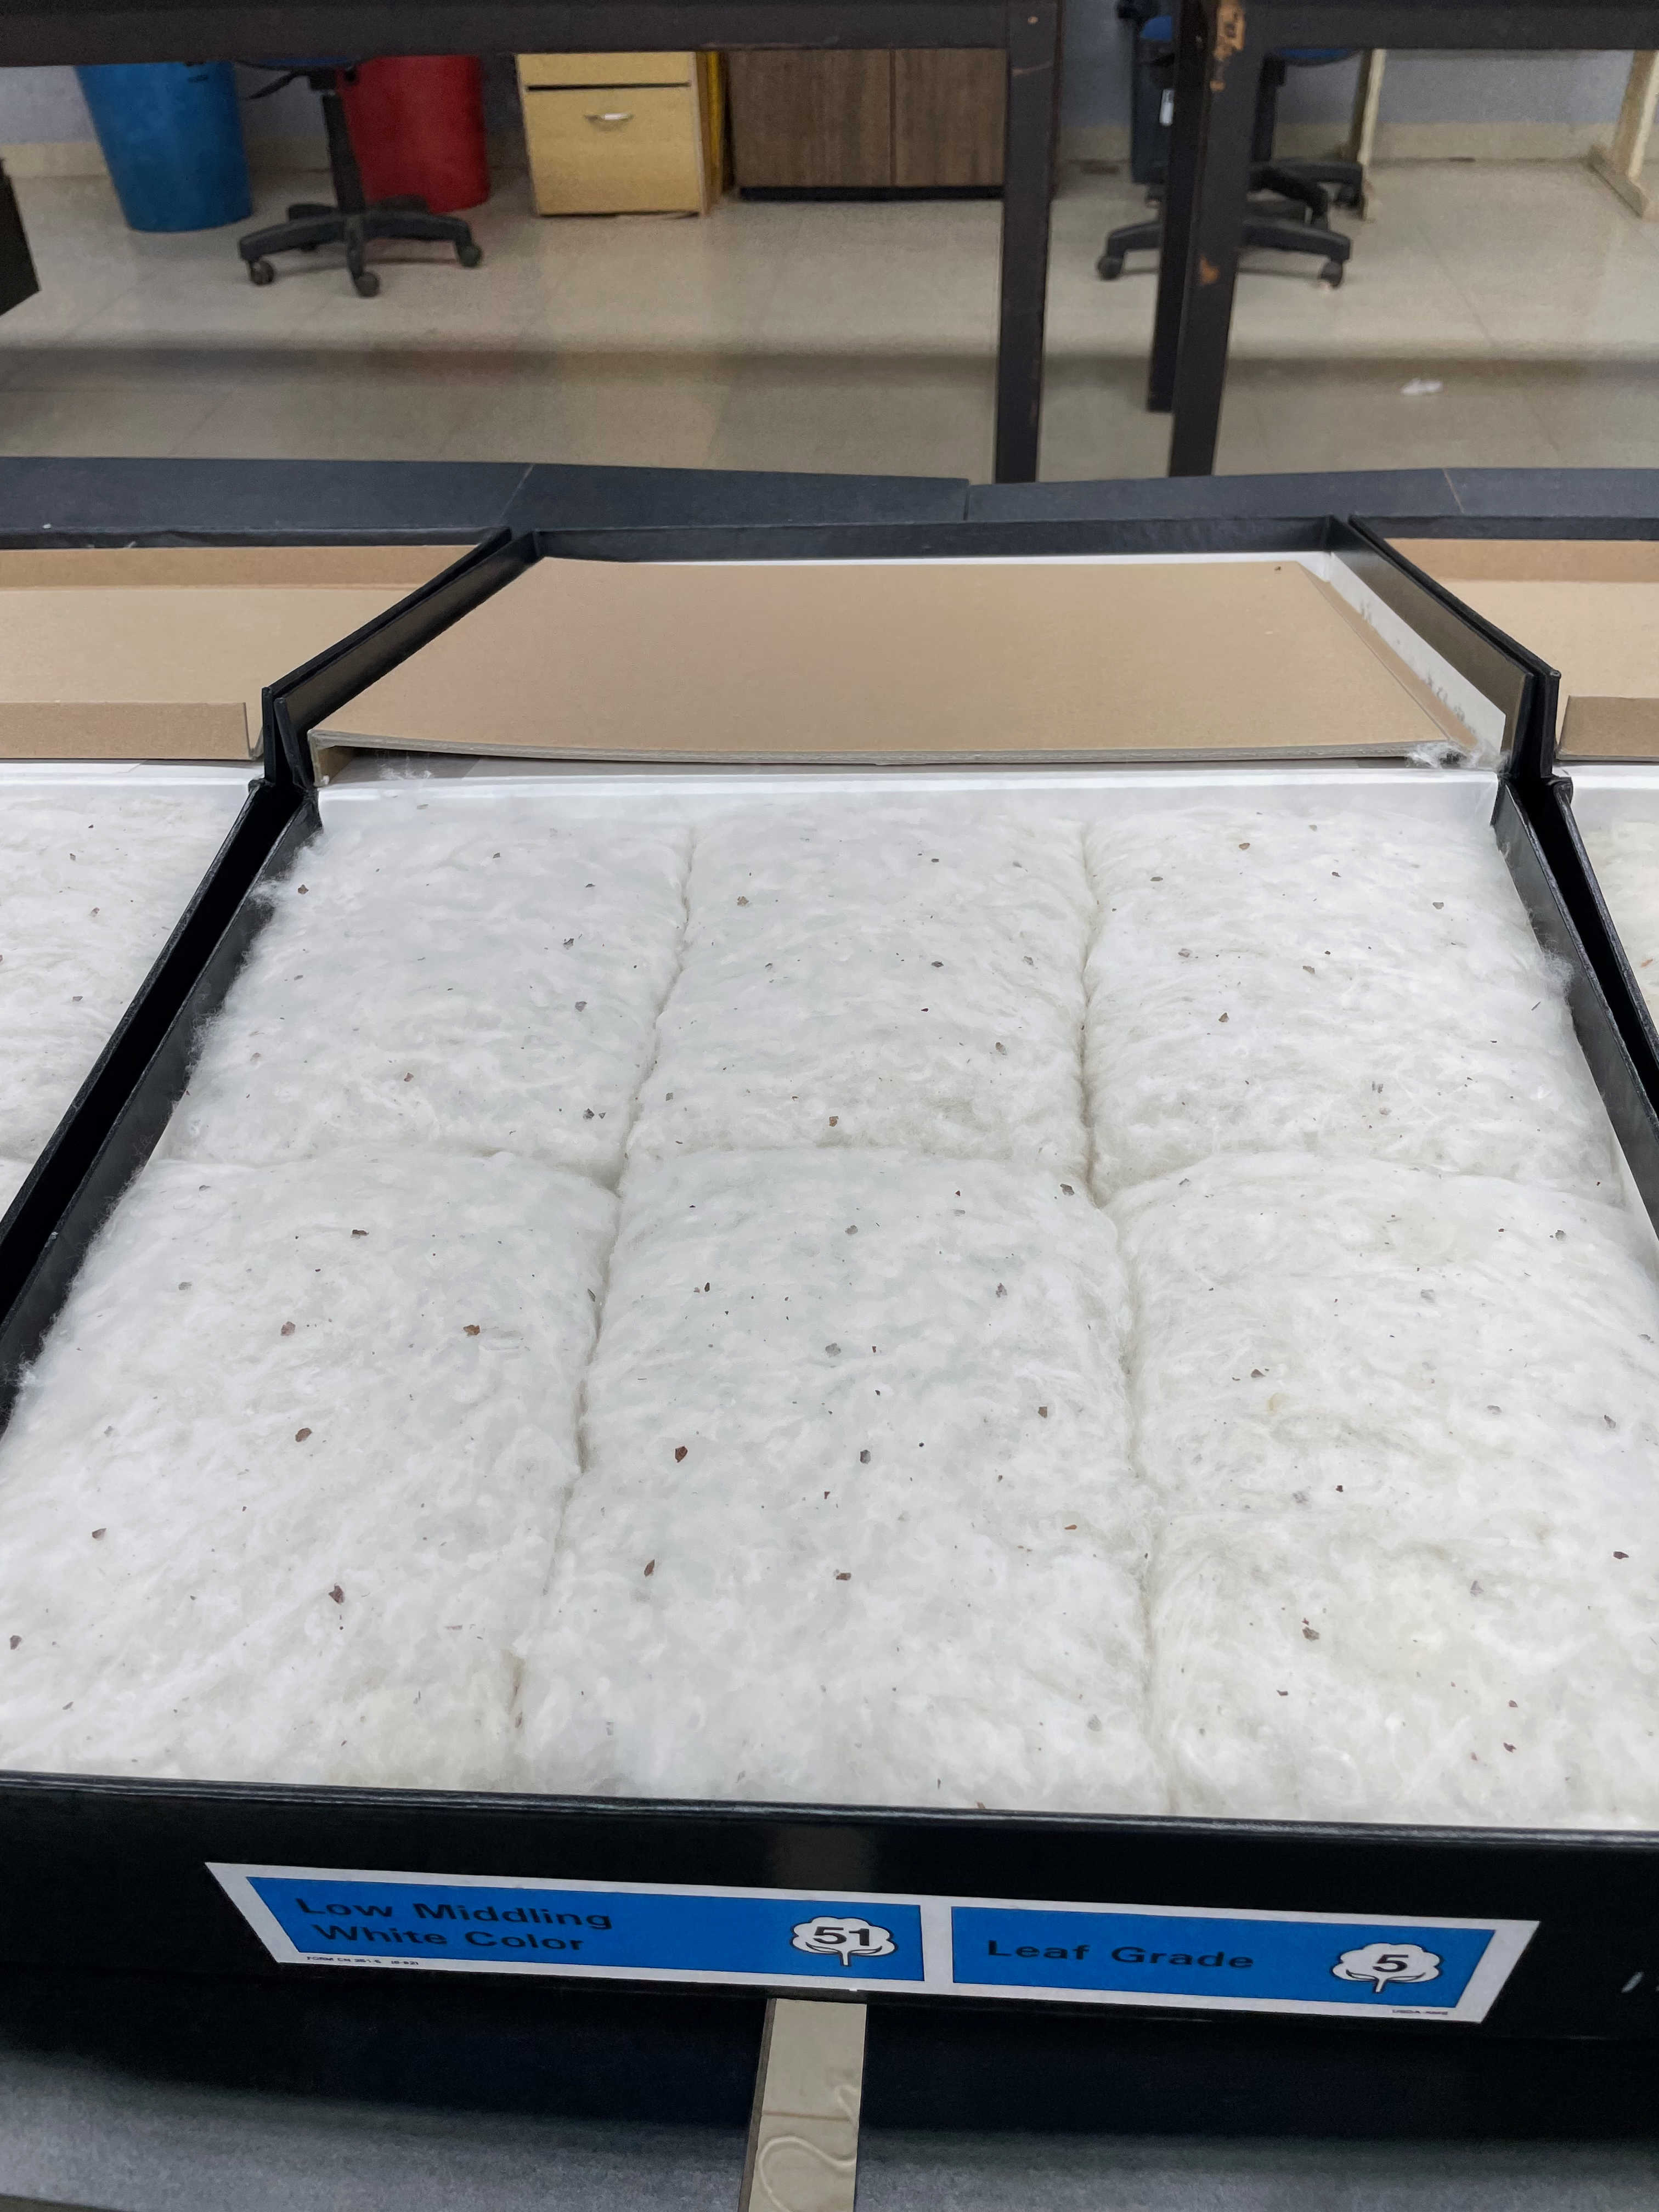
\includegraphics[trim={0 0 0 5cm},clip, scale=.3]{img/padrao_fisico_universal.jpeg}
	\end{center}
	\legend{Fonte: Do Autor}
\end{figure}

A classificação do algodão é feita com base em tipos de cor e graus de folha, ambos representados por códigos que correspondem aos Padrões Físicos Universais. A Tabela \ref{tab_tipo_cor} apresenta esses tipos de cor e suas respectivas classes. O grau de folha é uma escala que varia de 1 a 8, determinada pela quantidade de folhas presentes na amostra.  Esses padrões devem ser visualizados e memorizados antes de iniciar a classificação, pondendo ser consultados sempre que necessário.

Após a memorização dos padrões, as amostras devem ser divididas no sentido longitudinal ao meio, subdividindo as metades com cuidado para não descaracterizá-las durante o manuseio. As duas piores partes são selecionadas para análise, sendo a pior parte voltada para cima, para facilitar a análise.

Avalia-se a cor, brilho, manchas, impurezas, contaminações e defeitos de beneficiamento. A determinação do tipo é feita com base no Tipo de Cor e Grau de Folhas e o resultado é registrado no Laudo de Classificação.

\afterpage{%
    \clearpage% Flush earlier floats (otherwise order might not be correct)
    \thispagestyle{empty}% empty page style (?)
    \begin{landscape}% Landscape page
        \centering % Center table
        \begin{table}
            \centering
            \caption{Códigos dos tipos de Cor, Classes de Cor ou Grau de Cor do Algodão Upland}
            \begin{tblr}{
                width = \linewidth,
                colspec = {Q[l,m,400]Q[c,m,180]Q[c,m,220]Q[c,m,180]Q[c,m,220]Q[c,m,180]},
                row{1} = {font=\bfseries},
                vline{2-6} = {-}{},
                hline{3-9} = {-}{},
                hline{1-2,10} = {2pt}
              }
                                                                                  & Branco & Ligeiramente Creme & Creme & Avermelhado & Amarelado \\
              Cor Boa Média - GM (Good Middling)                         & 11              & 12                          & 13             & -                    & -                  \\
              Cor Estritamente Média-SM (Strict Middling)                & 21              & 22                          & 23             & 24                   & 25                 \\
              Cor Média-M (Middling)                                     & 31              & 32                          & 33             & 34                   & 35                 \\
              Cor Estritamente Abaixo da Média-SLM (Strict Low Middling) & 41              & 42                          & 43             & 44                   & -                  \\
              Cor Abaixo da Média-LM (Low Middling)                      & 51              & 52                          & 53             & 54                   & -                  \\
              Cor Estritamente Boa Comum-SGO (Strict Good Ordinary)      & 61              & 62                          & 63             & -                    & -                  \\
              Cor Boa Comum-GO (Good Ordinary)                           & 71              & -                           & -              & -                    & -                  \\
              Abaixo de Padrão                                           & 81              & 82                          & 83             & 84                   & 85                 
              \end{tblr}
        \label{tab_tipo_cor}
        \end{table}
    \end{landscape}
    \clearpage
}
\clearpage

\subsubsection{Classificação instrumental}

Em paralelo a segunda amostra é enviada para a classificação instrumental, que é realizada em laboratório. O ambiente de trabalho deve atender a condições específicas de umidade e temperatura. As amostras devem estar em bandejas teladas ou perfuradas em uma única camada para garantir circulação de ar.

São utilizados equipamentos do tipo HVI (\textit{High Volume Instrument}), que devem estar calibrados conforme as especificações do fabricante. Na Figura \Ref{fig_hvi_maquina}, é apresentado o modelo Uster HVI1000, que realiza a análise do HVI.

\begin{figure}[H]
	\caption{\label{fig_hvi_maquina}Equipamento Uster HVI 1000}
	\begin{center}
		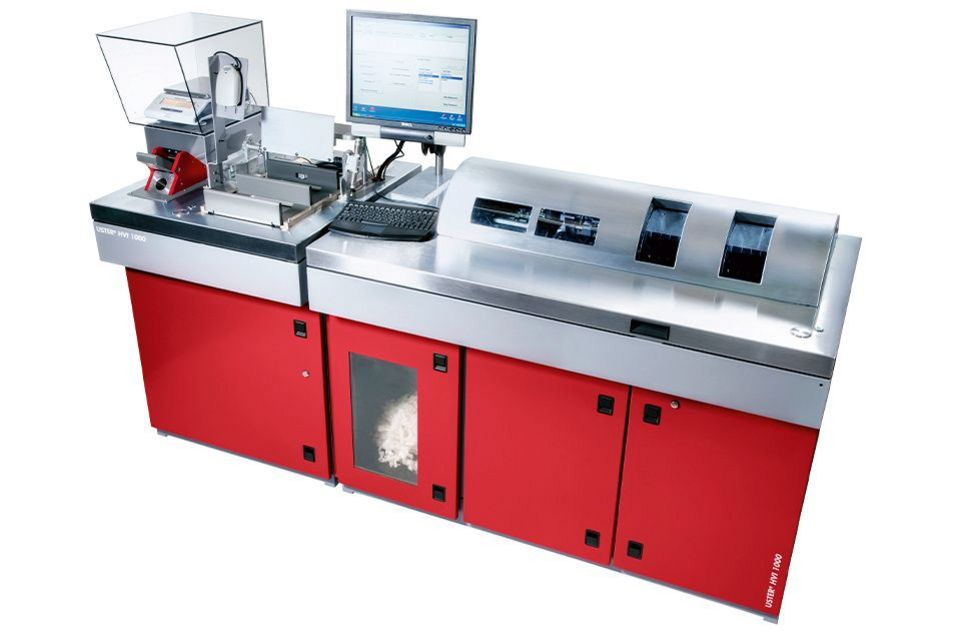
\includegraphics[trim={0 0 0 0},clip, scale=.3]{img/hvi_maquina.jpg}
	\end{center}
	\legend{Fonte: \cite{uster2024hvi}}
\end{figure}

O processo de análise consiste na análise de micronaire, que é feita em um corpo de prova, enquando os outros parâmetros são analisados em dois corpos de prova por amostra. A amostra é submetida ao equipamento HVI para obtenção do relatório. O resultado é analisado e um documento de classificação é gerado.

Os parâmetros analisados são:

\begin{itemize}
	\item Comprimento da Fibra (UHML): Comprimento médio da metade superior das fibras.
	\item Índice de Uniformidade do Comprimento da Fibra (\%UI): Relação entre o comprimento médio total das fibras e o comprimento médio das fibras mais longas.
	\item Resistência ou Tenacidade da Fibra (Str): Medida da força necessária para romper as fibras, expressa em gf/tex.
	\item Alongamento à Rotura da Fibra (\%Elg): Percentual de extensão que a fibra suporta antes de romper.
	\item Micronaire da Fibra (Mic): Combinação de finura e maturidade da fibra.
	\item Grau de Reflectância (\%Rd): Nível de luminosidade e cor branca refletida pelas fibras.
	\item Grau de Amarelamento (+b): Índice que expressa o nível de amarelamento da fibra.
	\item Índice de Fibras Curtas (\%SFI): Percentual de fibras com comprimento inferior a 0,50 polegadas.
	\item Índice de Consistência da Fiação (SCI): Valor calculado com base nas propriedades físicas das fibras e sua correlação com a performance de fiação.
\end{itemize}



\subsection{Relação entre a classificação visual e instrumental}
 
\citeonline{nickerson1958grade} chegaram à relação entre a reflectância (\%Rd) e o índice de amarelo (+b) com a classificação do algodão por meio de um estudo detalhado que utilizou o Colorímetro Nickerson-Hunter. Este instrumento mede a cor do algodão em termos destes dois atributos, permitindo uma representação em um gráfico bidimensional. Para converter essas medidas em uma classificação de cor única, os autores desenvolveram um índice que relaciona os valores medidos com os padrões oficiais de tipo de algodão. 

A análise envolveu encontrar uma linha de melhor ajuste entre os dados medidos e os padrões de cor, utilizando métodos de regressão para obter fórmulas de conversão e diagramas que facilitassem essa associação (Figura \ref{fig_hvi_color_chart}). Essa abordagem permitiu criar índices numéricos para diferentes estados do algodão, como fibras em estado bruto e fios tingidos, mantendo o valor de \textit{Middling} (Cor Média) em 100 e ajustando as relações para outros graus de cor.

\clearpage
\begin{figure}[H]
	\caption{\label{fig_hvi_color_chart}Gráfico de cores e classificação manual e instrumental de fibras de algodão. No eixo vertical, estão os valores de reflectância. Quanto maior o valor, mais brilhante é o algodão. No eixo horizontal, estão valores típicos do índice de amarelo. Quanto maior o valor, mais amarela é a amostra.}
	\begin{center}
		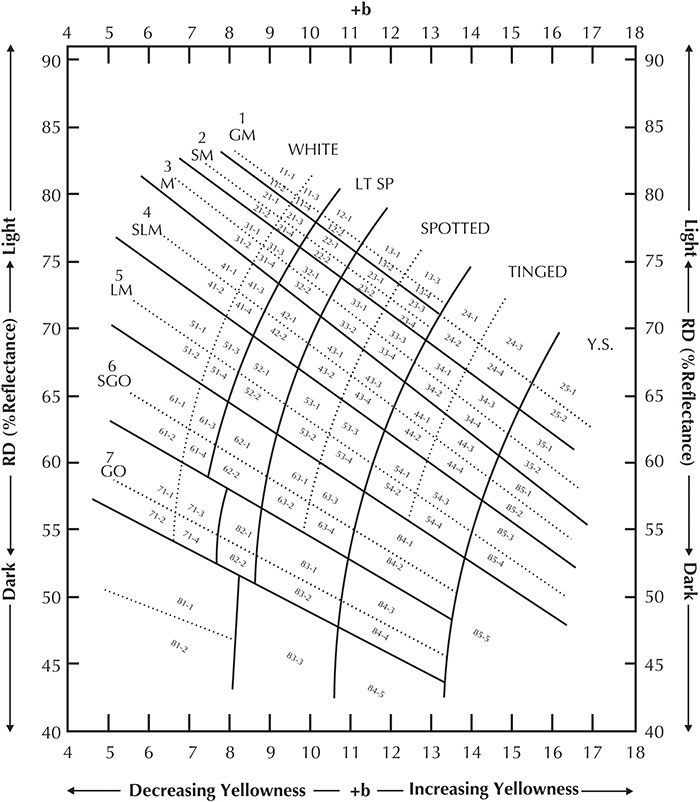
\includegraphics[trim={0 0 0 0},clip, scale=.5]{img/hvi_color_chart.jpg}
	\end{center}
	\legend{Fonte: \citeonline{cottoninc2024hvicolor}}
	% \nota{}
\end{figure}


\section{Visão Computacional}\label{rev_cv}

Neste capítulo será explorada com mais profundidade a disciplina de visão computacional, os sistemas de visão computacional e seus conceitos fundamentais, o processamento de imagens e aplicação da visão computacional no agro, com ênfase nas tecnologias e métodos aplicados à cultura do algodão.

\citeonline{oliveira2024visao} descrevem o histórico da visão computacional como uma ciência recente, cuja primeira menção foi em 1955, com a ideia de equipar computadores com "olhos e ouvidos". Na década de 1970, os primeiros estudos combinaram visão computacional com inteligência artificial, acreditando que a emulação da visão humana por máquinas seria rapidamente alcançada. Destaque para \citeonline{marr1976vision} que, dentro do campo da neurofosiologia, desenvolveu uma abordagem computacional para a visão, que consistia na formulação de um algoritmo para interpretação visual em qualquer contexto físico. Seus estudos foram um dos principais pontos de partida para as pesquisas em visão computacional \cite{vaina2004marr}.

No entanto, descobriu-se que a complexidade era maior do que imaginado, devido à falta de informações sobre a interpretação de imagens pelo cérebro humano, levando a avanços progressivos nas décadas seguintes \cite{oliveira2024visao}, resultando na consolidação da visão computacional como a disciplina que busca desenvolver métodos e algoritmos para que os computadores possam interpretar e entender imagens de forma semelhante à percepção humana \cite{ballard1982computer}.

\subsection{Sistemas de visão computacional}

\citeonline{saldana2013review} discute que os sistemas de visão computacional são projetados para extrair e analisar informações de objetos de forma automática e objetiva, sendo rápidos, consistentes e não invasivos. Esses sistemas geralmente consistem em um dispositivo de captura de imagens, dispositivo de iluminação e um computador que processa as imagens capturadas.

\subsubsection{Captura de imagens}

Existem diferentes sensores que podem ser utilizados para gerar uma imagem, como ultrassom, raios-X, sensores térmicos, sensores de espectroscopia de infravermelho próximo (NIR) e câmeras tradicionais, estas geralmente mais utilizadas em problemas de visão computacional \cite{brosnan2004improving}. 

As câmeras são responsáveis pela captura da imagem, que é então convertida em sinais eletrônicos e processada. Basicamente, existem dois tipos de sersores: as câmeras CCD (\textit{Charge-Coupled Device}) e CMOS (\textit{Complementary Metal-Oxide-Semiconductor}).

As câmeras CCD são reconhecidas pela alta qualidade de imagem que oferecem, especialmente em condições de baixa iluminação. Isso ocorre devido ao menor ruído intrínseco de seus sensores, que apresentam substratos mais silenciosos e menor quantidade de circuitos integrados no chip. Além disso, os sensores CCD possuem maior faixa dinâmica, proporcionando uma melhor relação entre os níveis de saturação e o limite inferior de sinal detectável, o que resulta em imagens mais detalhadas e com melhor gradação tonal. Outra vantagem significativa das câmeras CCD é a uniformidade na resposta dos pixels, o que as torna ideais para aplicações que exigem alta precisão, como fotografia científica, televisores de alta performance e aplicações médicas. No entanto, essa tecnologia apresenta desvantagens como maior consumo de energia e tamanho físico do sistema, já que muitas funções do sensor dependem de circuitos externos \cite{littwiller2001ccd_cmos}.

Os sensores CMOS evoluíram significativamente nas últimas décadas, consolidando-se como uma alternativa viável aos CCDs, especialmente em aplicações que demandam baixo custo, baixo consumo de energia e integração de múltiplas funcionalidades em um único chip. A arquitetura CMOS permite a integração de circuitos analógicos e digitais diretamente no sensor, resultando em sistemas menores e mais leves. Além disso, sensores CMOS consomem menos energia, podendo operar com uma única fonte de baixa tensão, o que os torna ideais para dispositivos móveis e portáteis. Apesar dessas vantagens, os CMOS ainda enfrentam desafios como menor sensibilidade, maior ruído em condições de baixa iluminação e menor faixa dinâmica \cite{bigas2006cmos}. Na Tabela \ref{tab:ccd_vs_cmos} é apresentado um resumo comparando as principais características dos sensores CCD e CMOS, apresentados por \citeonline{bigas2006cmos}.

\begin{table}[ht]
    \centering
    \caption{Resumo comparativos das principais características entre sensores CCD e CMOS}
    \begin{tabular}{l|c|c}
    \hline
    \textbf{Característica}             & \textbf{CCD}                  & \textbf{CMOS}                  \\ \hline
    Consumo de energia                  & Alto                          & Baixo                          \\ 
    Custo                               & Alto                          & Baixo                          \\ 
    Integração em chip                  & Não                           & Sim                            \\ 
    Flexibilidade                       & Limitada                      & Alta                           \\ 
    Faixa dinâmica                      & Alta                          & Limitada                       \\ 
    Sensibilidade                       & Alta                          & Limitada                       \\ 
    Ruído                               & Baixo                         & Alto                           \\ 
    Qualidade de imagem                 & Alta                          & Limitada                       \\ 
    Velocidade                          & Limitada                      & Alta                           \\ 
    Tamanho físico do sistema           & Maior                         & Menor                          \\ 
    Aplicações                          & Alta qualidade, ciências      & Dispositivos móveis, segurança \\ \hline
    \end{tabular}
    \label{tab:ccd_vs_cmos}
    \legend{Fonte: \citeonline{bigas2006cmos}}
\end{table}

FALAR AQUI SOBRE FORMA DE TRANSMITIR IMAGENS E COMPACTAÇÃO JPG E BMP

\subsubsection{Iluminação}

A iluminação desempenha um papel essencial nos sistemas de visão computacional, pois define as propriedades ópticas dos objetos a serem analisados. A luz incidente pode ser absorvida, refletida ou transmitida, influenciando diretamente a qualidade das imagens capturadas. Para otimizar o desempenho do sistema de visão, a escolha e a configuração do sistema de iluminação devem ser adaptadas à aplicação específica. Essa seleção cuidadosa reduz a necessidade de etapas complexas de processamento de imagem, aumentando a eficiência e a precisão das análises \cite{chen2002machine_vision}.

\citeonline{zhang2014computer} destacam a importância de fontes de luz que realcem as características dos objetos e permitam distinções claras entre as partes detectadas e outras áreas. A eficiência e a precisão de um sistema de visão computacional dependem significativamente da qualidade da iluminação, que deve fornecer luz uniforme e estável, além de evitar reflexos e sombras que possam comprometer a análise. 

A escolha da iluminação ideal depende das características espectrais desejadas para a aplicação, considerando tanto a geometria do objeto quanto os atributos a serem destacados. Por exemplo, sistemas que utilizam luz difusa são eficazes para minimizar reflexos especulares, enquanto a iluminação traseira pode ser essencial para delinear contornos e aumentar o contraste em objetos translúcidos. Diferentes tipos de lâmpadas são utilizados, incluindo tubos de raios X, fluorescentes, incandescentes, lasers e lâmpadas de infravermelho, cada uma operando em faixas espectrais específicas, desde raios X (0,01-10 nm) até o infravermelho próximo (700-2500 nm). Enquanto as lâmpadas fluorescentes são preferidas para análises baseadas em luz visível, os LEDs têm ganhado destaque por sua estabilidade, baixo consumo de energia e ampla disponibilidade em comprimentos de onda específicos \cite{cubero2010advances}.

\subsubsection{Software}

????

\subsection{Processamento e análise de imagens}

O processamento e a análise das imagens são componentes fundamentais nos sistemas de visão computacional, desempenhando um papel crucial na extração de informações visuais úteis para a classificação, detecção de defeitos e avaliação de qualidade \cite{krutz2000colour}. 

Segundo \citeonline{brosnan2002}, o processamento de imagens engloba operações destinadas a melhorar a qualidade das imagens capturadas, removendo ruídos, corrigindo distorções geométricas e uniformizando a iluminação. Essas etapas iniciais são essenciais para garantir que as imagens estejam adequadamente preparadas para a análise subsequente. Já a análise de imagens refere-se à segmentação e à extração de características dos objetos de interesse, como forma, cor e textura, permitindo a interpretação e o reconhecimento dos elementos nas imagens.

O processamento/análise de imagens é frequentemente dividid0 em três níveis: o processamento de baixo nível, que inclui a aquisição e o pré-processamento de imagens; o processamento de nível intermediário, focado na segmentação, representação e descrição; e o processamento de alto nível, que envolve o reconhecimento e a interpretação de padrões \cite{gunasekaran1996computer, sun2000pizza}.

A aquisição consiste na conversão do sinal eletrônico do sensor para uma forma numérica. O pré-processamento refere-se ao processamento inicial dos dados brutos da imagem para correção de distorções geométricas, remoção de ruídos, correção do nível de cinza e correção de desfoque \cite{shirai1987}. O objetivo dessa etapa é melhorar a qualidade da imagem, removendo distorções indesejadas ou destacando características de interesse.

No nível intermediário, a segmentação de imagens é uma das etapas mais importantes em toda a técnica de processamento de imagens, pois os dados extraídos posteriormente dependem fortemente da precisão dessa operação. Seu principal objetivo é dividir uma imagem em regiões que possuam uma forte correlação com objetos ou áreas de interesse. A segmentação pode ser realizada por três técnicas diferentes: limiarização, segmentação baseada em bordas e segmentação baseada em regiões. A representação se refere à maneira como a forma ou estrutura de um objeto é modelada e armazenada, seja por contornos, áreas, momentos ou outras técnicas que traduzem os dados visuais para formatos matemáticos ou computacionais. Descrição, por sua vez, é o processo de derivar atributos ou características mensuráveis a partir dessa representação, como tamanho, forma, textura ou relações espaciais, que podem ser usadas para classificação, reconhecimento ou análise mais profunda \cite{sonka1993}.

O processamento de alto nível envolve o reconhecimento e interpretação de padrões, que visam a transformação de dados visuais em informações compreensíveis. \citeonline{sonka1993} trazem também que o reconhecimento de padrões refere-se à identificação de objetos ou estruturas em uma imagem com base em suas características distintivas, utilizando métodos como aprendizado estatístico, redes neurais, e técnicas sintáticas para classificar ou agrupar dados visuais. Já a interpretação de padrões vai além, envolvendo o uso de conhecimento contextual e estratégias hierárquicas para compreender o significado dos objetos reconhecidos e suas relações no ambiente analisado.

\subsection{Aplicações da visão computacional no Agronegócio}

A visão computacional tem desempenhado um papel fundamental no agronegócio, sendo aplicada em áreas como classificação de culturas, detecção de doenças, monitoramento de qualidade, automação de processos e muito mais. A seguir, apresentam-se os principais estudos categorizados por aplicação.

\subsubsection{Classificação e Qualidade de Fibras}
\cite{li2023} propuseram algoritmos para medir a cor do algodão em pluma, corrigindo distorções e melhorando a classificação de qualidade.  
% \citet{Niloy2024} desenvolveram o dataset \textit{CottonFabricImageBD}, utilizando redes neurais para quantificar o percentual de algodão em tecidos.  
% \citet{Thomasson2005} abordaram problemas de medição de cor no algodão, utilizando câmeras e algoritmos avançados de segmentação.  
% \citet{Oliveira2022} utilizaram espectroscopia Raman portátil para classificar fibras de algodão por localidade, maturidade e modificação genética.  
% \citet{Fisher2022} aplicaram aprendizado de máquina para classificar fibras de algodão egípcio, alcançando precisão de 90\%.  
% \citet{Cheng1999} propuseram um sistema híbrido de lógica fuzzy e redes neurais para classificar a cor do algodão, melhorando a consistência com classificações humanas.  
% \citet{Matusiak2010} exploraram técnicas de medição de cor instrumental para algodão, destacando os desafios em igualar a precisão da classificação humana.  
% \citet{Zayas1996} apresentaram métodos baseados em textura para classificar variedades de trigo e outros cereais, utilizando visão computacional em sistemas de qualidade.  
% \citet{Ghazal2024} revisaram abordagens em precisão agrícola com UAVs para análise de qualidade e mapeamento de zonas de manejo.  
% \citet{Wang2024} aplicaram redes convolucionais para detectar fibras contaminantes no algodão, aumentando a eficiência em sistemas automatizados.  

% \subsubsection{Detecção de Doenças em Plantas}
% \citet{Ahad2023} implementaram arquiteturas CNN para detectar doenças em folhas de arroz, com acurácia superior a 98\%.  
% \citet{Ritharson2024} introduziram o modelo \textit{DeepRice}, com precisão de 99.94\% para identificação precoce de doenças críticas.  
% \citet{Shwetha2024} apresentaram o \textit{LeafSpotNet}, otimizando o desempenho para dispositivos móveis.  
% \citet{Paymode2022} destacaram o uso de transfer learning na classificação de doenças foliares em múltiplas culturas.  
% \citet{Ding2024} revisaram métodos baseados em CNN e Transformers para detecção de doenças em culturas agrícolas.  
% \citet{Zhu2014} aplicaram algoritmos baseados em saliência para análise e detecção de resíduos foliares, melhorando a eficiência na segmentação.  

% \subsubsection{Monitoramento e Contagem de Culturas}
% \citet{Jiang2024} usaram UAVs e YOLOv8 para detecção e contagem de melancias em campo.  
% \citet{Singh2023} desenvolveram algoritmos leves para identificar bolas de algodão durante a colheita automatizada.  
% \citet{Guo2024} apresentaram uma abordagem baseada em Unet para detecção de linhas de cultivo, melhorando a navegação em sistemas autônomos.  

% \subsubsection{Classificação de Grãos e Frutas}
% \citet{Majumdar1999} introduziram técnicas de análise de textura para classificar cereais, atingindo 100\% de precisão.  
% \citet{Utku2000} usaram seleção de características para classificar variedades de trigo.  
% \citet{Zhu2024} desenvolveram métodos de luz estruturada para detectar danos em maçãs, alcançando métricas IoU superiores a 91\%.  

% \subsubsection{Detecção de Matérias Estranhas e Ervas Daninhas}
% \citet{Zhang2014} revisaram aplicações de visão computacional na detecção de resíduos em algodão.  
% \citet{Wang2023} implementaram YOLOv5 para identificar contaminantes no algodão.  
% \citet{Juwono2023} revisaram técnicas de aprendizado de máquina para separar ervas daninhas de culturas.  
% \citet{Subeesh2022} alcançaram 97.7\% de precisão na identificação de ervas daninhas com InceptionV3.  
% \citet{Ramos2024} implementaram YOLOv8 para detectar fumaça e incêndios florestais, com implicações para segurança agrícola.  

% \subsubsection{Automação e Previsão de Parâmetros de Animais}
% \citet{Klancar2004} projetaram sistemas de visão global para robôs agrícolas, otimizando navegação e análise em campo.  
% \citet{Xie2024} usaram o Mask R-CNN para prever peso de suínos em fazendas automatizadas.  
% \citet{Chuquimarca2024} revisaram técnicas de CNN para classificação de frutas com dados hiperespectrais.  
% \citet{Ramos2024} destacaram o uso de YOLOv8 em sistemas de monitoramento ambiental para identificação de riscos.  
% \citet{Ghazal2024} propuseram novas metodologias baseadas em visão computacional para integrar mapas de precisão com estratégias de manejo.  
% \citet{Patricio2018} revisaram tecnologias de visão computacional para monitoramento de grãos, abordando impactos em sustentabilidade.  




\section{Inteligência Artificial}\label{rev_ia}

\begin{itemize}
	\item Contextualizar o que é IA
	\item Modelos de imagem
	\item PCANet
	\item VGGNEt
	\item CNN
	\item SVM
	\item ???
\end{itemize}



\section{Lacunas na Literatura}\label{rev_lacunas}

\chapter{Metodologia}\label{metodologia}

\chapter{Resultados Esperados}\label{result}

\chapter{Discussão}\label{discussao}